% pdflatex -shell-escape ignore.parts.tex
%\documentclass[convert={ghostscript,density=480,outname=parts,outext=.png}]{standalone}
\documentclass[convert={command=\unexpanded{pdf2svg \infile\space\outfile},outname=parts,outext=.svg}]{standalone}
\usepackage{tikz}
\usepackage{graphicx}
\usetikzlibrary{calc}

\begin{document}
    \begin{tikzpicture}
        \node [above right, inner sep=0] (image) at (0,0) {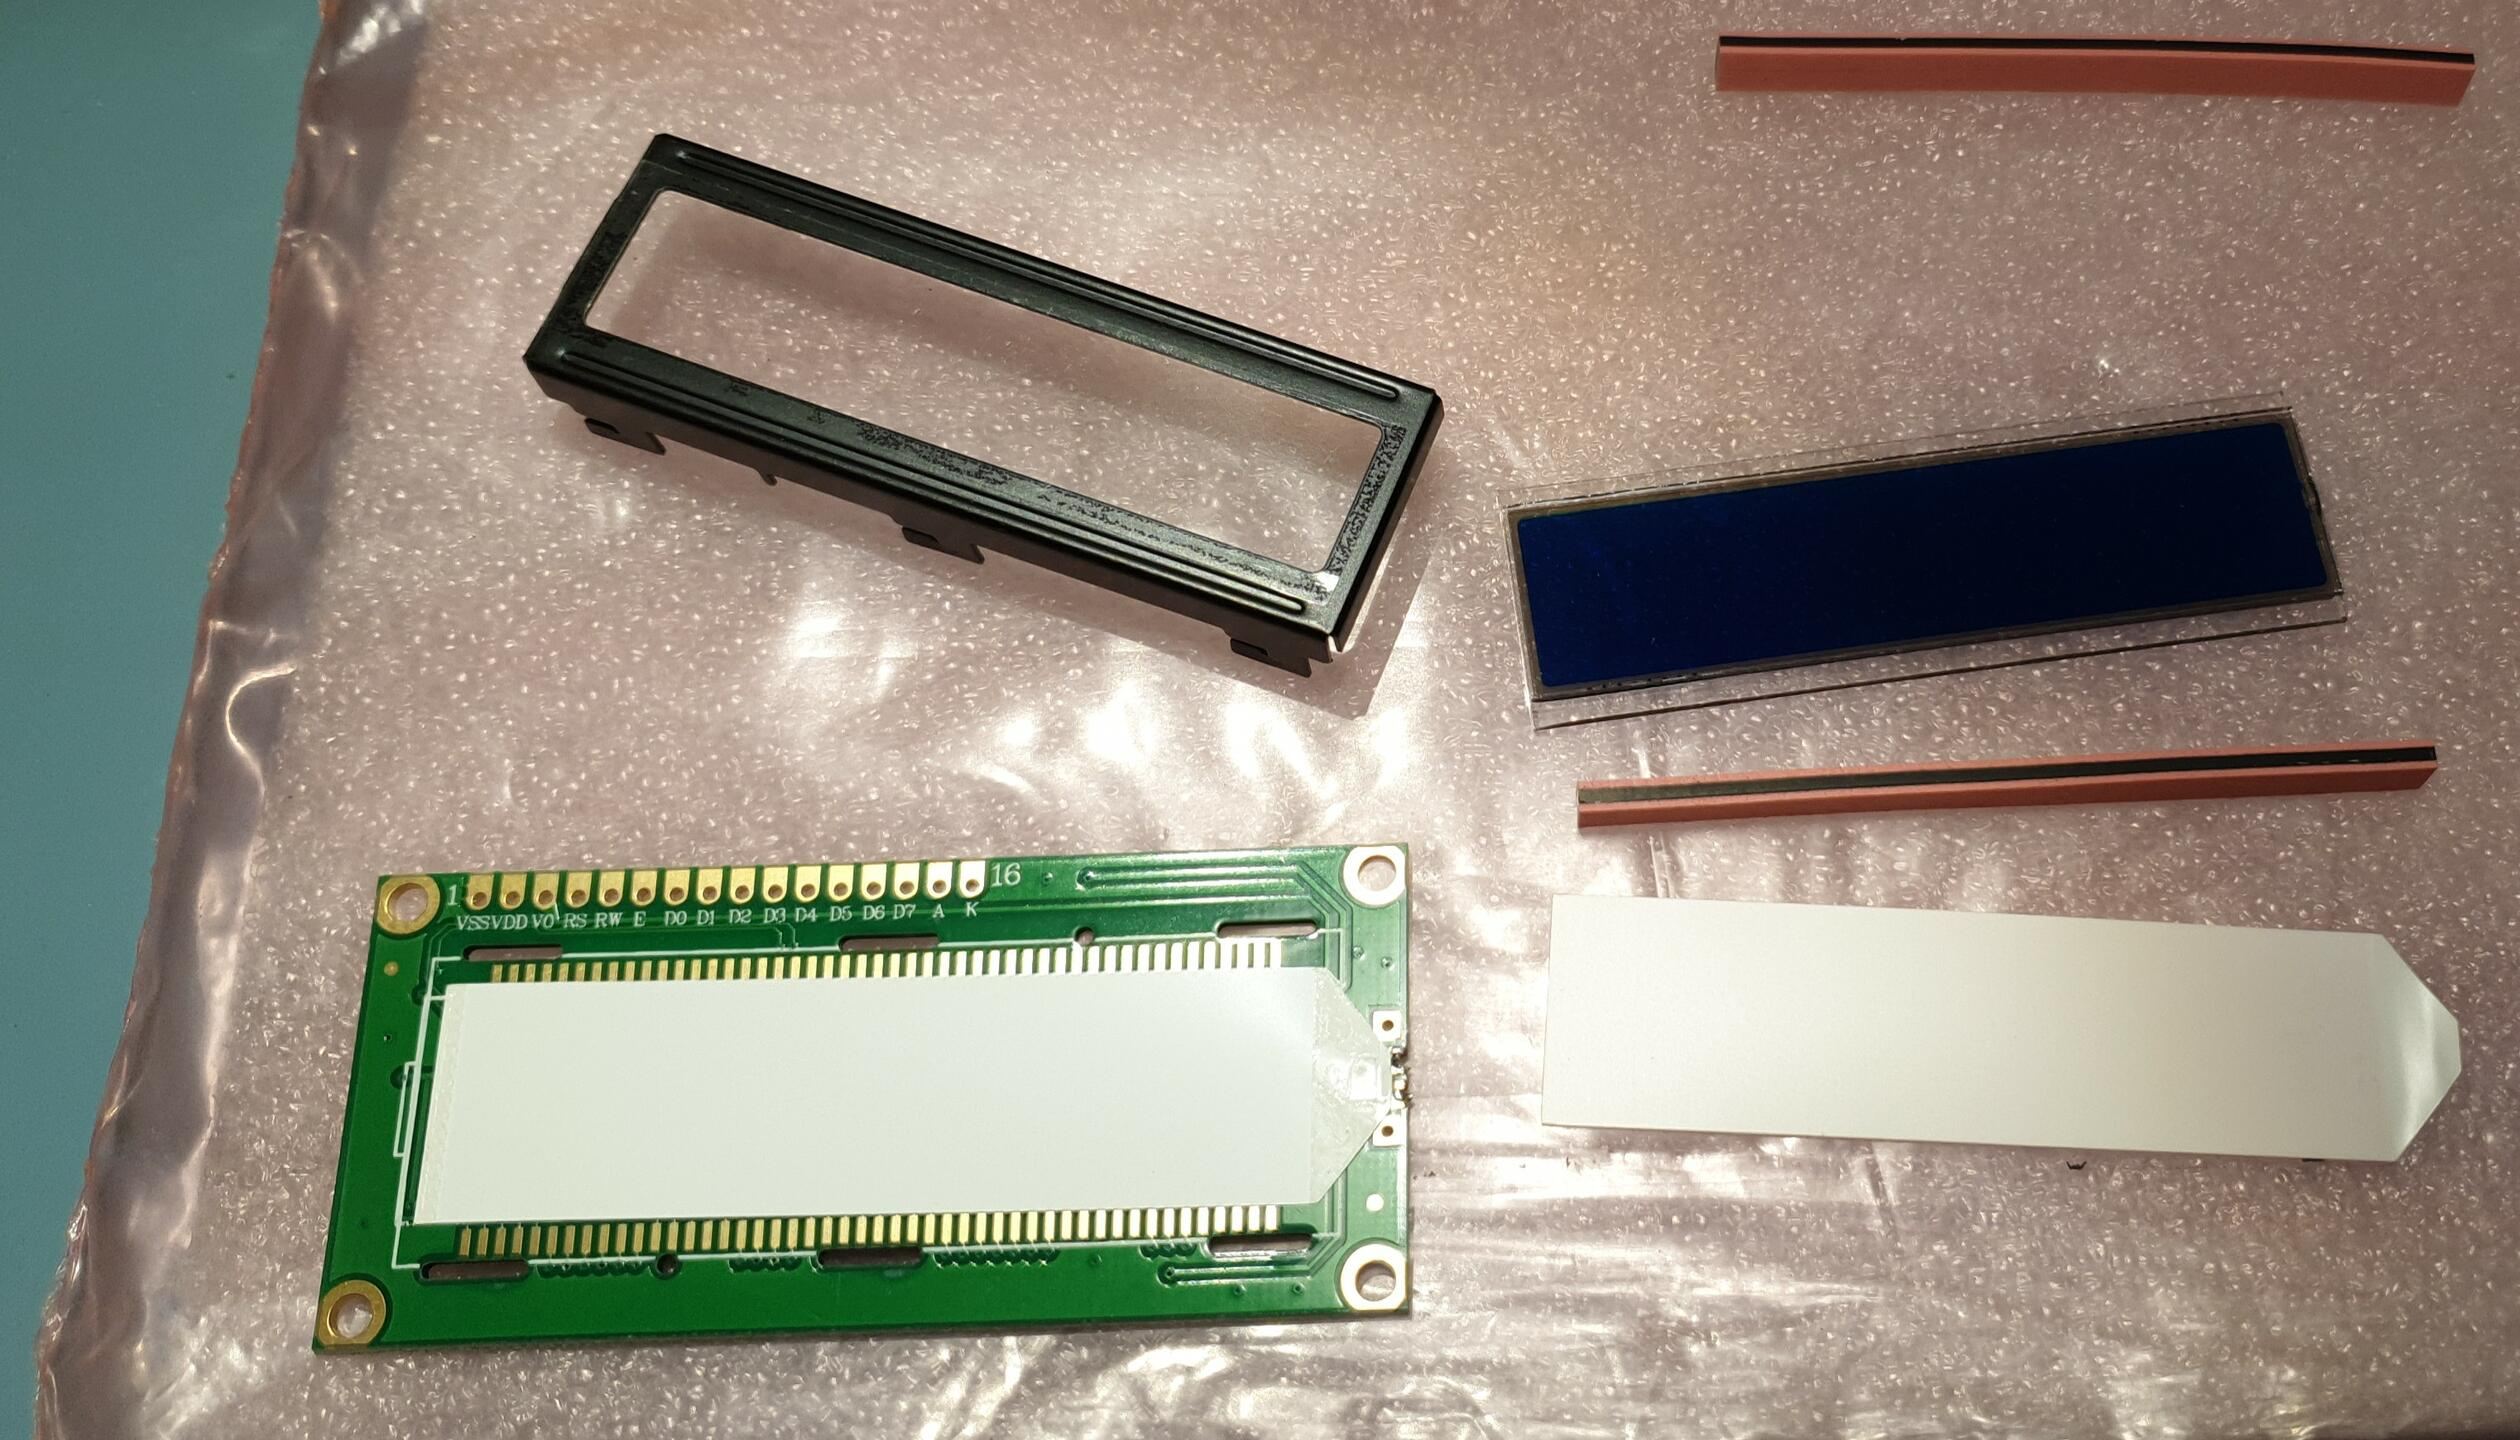
\includegraphics[width=\textwidth]{ignore.parts.jpg}};

        \begin{scope}[
            x={($1*(image.south east)$)},
            y={($1*(image.north west)$)}
        ]
            % grid
            %\draw[lightgray,step=0.1] (image.south west) grid (image.north east);

            \draw[stealth-, very thick,green] (0.5,0.2) -- ++(0.10,-0.10)
                node[right,black,fill=white]{\small lower BLU sheet (reflector)};

            \draw[stealth-, very thick,green] (0.9,0.24) -- ++(-0.02,-0.06)
                node[left,black,fill=white]{\small upper BLU sheet};

            \draw[very thick,green] (0.10,0.05) rectangle (0.58,0.45)
                node[below left,black,fill=white]{\small PCB};

            \draw[very thick,green] (0.59,0.48) rectangle (0.95,0.80)
                node[below left,black,fill=white]{\small open cell};

            \draw[very thick,green] (0.20,0.50) rectangle (0.58,0.92)
                node[below left,black,fill=white]{\small frame};

            \draw[latex-, very thick, green] (0.70,0.95) edge (0.60,0.97)
                (0.65,0.45) -- (0.60,0.97)
                node[left,black,fill=white]{\small Zebra strips};

            \node at (1,0) [above left, black,fill=white] {Missing in the picture is the BLU light guide plate.};
        \end{scope}
    \end{tikzpicture}
\end{document}
